% !TEX root = LMEDS_manual.tex

%%%%%%%%%%%%%%%%%%%%%
\section{Orientation}
%%%%%%%%%%%%%%%%%%%%%

LMEDS comes packaged with the following folders:

\begin{itemize}
\item cgi-bin

Small code snippets (with the extension .cgi) go here--one for each experiment

\item html

Contains static HTML, Javascript, and CSS files

\item imgs

Image files used by LMEDS

\item lmeds

The main repository for code.

\item lmeds/user\_scripts

Within the lmeds code directory are some scripts that users can use in setting up their experiments and in post-processing their data.

\item tests

Holds the resource files for each experiment

\item user\_manual

Contains the user manual

\end{itemize}

\paragraph{}

If you are creating an experiment, you'll need to add one file to cgi-bin and you'll need to add a folder to tests, containing all of the resource files used in the experiment--the other folders can all be ignored. The next section goes into the details of how to create the 

\subsection{Getting started with LMEDS}

This manual describes how to create files used by LMEDS from scratch.  You might find it useful to reference the experiment files that come with LMEDS, located in /tests/lmeds\_demo.  In it, you'll find an example dictionary (english.txt), sequence file (sequence.txt), input files contained in the (audio/ and txt/ folders), survey files (presurvey.txt and postsurvey.txt), and some sample output files (stored in the folder output/).
\textbf{When you are starting a new experiment from scratch, you might find it useful to start with the demo files provided.}

\begin{figure}
\subsection{LMEDS Workflow Schematic}
\centering
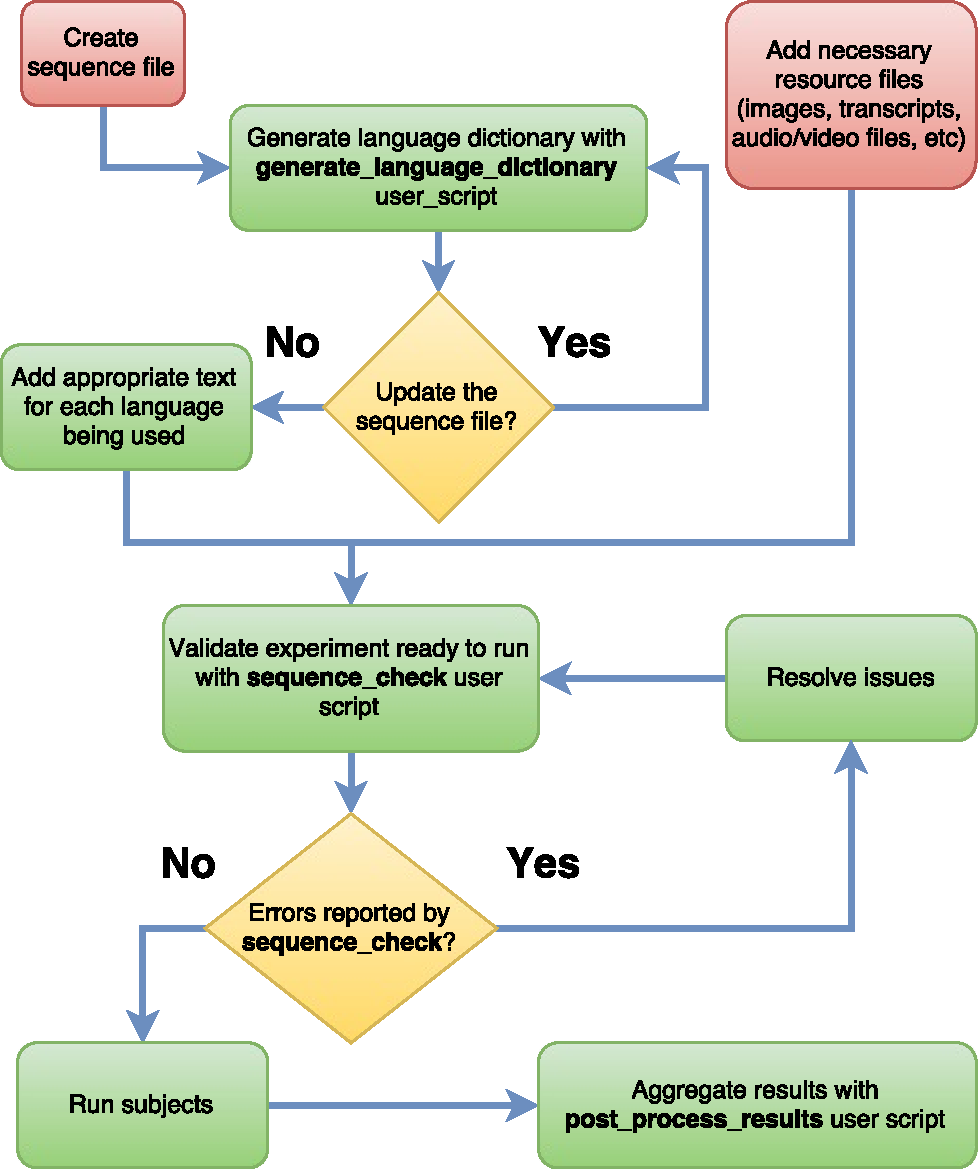
\includegraphics[height=0.95\textheight]{lmedsSchematic.pdf}
\end{figure}


\paragraph{}

To begin an LMEDS experiment, two things are needed--resource files and a sequence file (the two boxes in red).  Once the sequence file is sufficient for your purposes, a language dictionary is generated from it with the user script generate\_language\_dictionary.  If any changes are made to the sequence file, the language dictionary will need to be regenerated.  Once the sequence file and language dictionary are syncronized, enter the appropriate text for each language being used.

\paragraph{}
With the sequence files, resource files, and generated language dictionary, validate that the experiment can be run using sequence\_check.  sequence\_check will ensure that all resources and text specified in the sequence file are available and that each page in the sequence file can be created.  As long as there are issues, resolve them and run the script again.  Once there are no reported errors, test it for yourself and then run subjects.  After collecting all subject data, use post\_process\_results to aggregate the user data.



